\documentclass[a4paper,12pt]{article}
\usepackage[utf8]{inputenc}
\usepackage[margin=3cm]{geometry}
\usepackage{amsmath}
\usepackage{amssymb}
\usepackage{amsthm}
\usepackage{fancyhdr}
\usepackage{seminar}
\usepackage{graphicx}
\usepackage{subfigure}
\usepackage{float}
\usepackage{hyperref}
\pagestyle{fancy}


%You can add theorem-like environments (e.g. remark, definition, ...) if you want
\newtheorem{theorem}{Theorem}

\title{Seminar Report of KinectFusion: Real-Time\\Dense Surface Mapping and Tracking} % Replace with your title
\author{Wenliang Peng} % Replace with your name
\institute{Faculty of Informatics - Technische Universit\"{a}t M\"{u}nchen} % Replace with the department you belong to

\makeatletter
\let\runauthor\@author
\let\runtitle\@title
\makeatother
\lhead{\runauthor}
\rhead{\runtitle}


\begin{document}

\maketitle

\begin{abstract}
	The paper "KinectFusion: Real-Time Dense Surface Mapping and Tracking" was published by Microsoft Research and was published in 2011. 
	The method proposed in this paper is a pioneering work based on a low-cost RGB-D camera for real-time reconstruction tracking and reconstruction. 
	And it is an algorithm suitable for different lighting conditions, creating an important framework for 3D dense reconstruction. 
	This paper shows that this method can accurately obtain tracking and mapping results in real-time in room-sized scenes using only commodity sensors and GPU hardware, which surpassed the solutions proposed using passive computer vision at that time.
\end{abstract}

\section{Introduction}

In computer vision, research on structure from motion (SFM) and multi-view stereo (MVS) has produced many compelling results. 
However, much of this work was not motivated by real-time applications. 
Simultaneous localization and mapping (SLAM) research focuses more on real-time unmarked tracking and real-time scene reconstruction based on monocular RGB camera input. 
However, although these systems perform real-time mapping, they are optimized for effective camera tracking, and the sparse point cloud models they produce can only perform basic scene reconstruction.
With the advent of Microsoft Kinect, this highly cost-effective camera with a depth sensor can provide opportunities for SLAM and AR.
This article propose a detailed method that allows the use of handheld Kinect depth sensors to perform real-time, dense volumetric reconstruction of complex room-sized scenes. 
The use of highly parallel general-purpose GPU (GPGPU) technology is at the core of all our design decisions. It allows tracking and mapping to be performed at the frame rate of the Kinect sensor and in constant time\cite{6162880}.

\section{Method description}
In this method, a dense reconstruction algorithm using depth maps is created to accurately reconstruct the 3D model in real-time. 
the algorithm pipeline is shown in Figure \ref{figure1}, 
including four parts, namely measurement, pose estimation, reconstruction update, and surface prediction.
\begin{figure}[h] %figure环境,h默认参数是可以浮动,不是固定在当前位置。如果要不浮动,你就可以使用大写float宏包的H参数,固定图片在当前位置,禁止浮动。
    \centering %使图片居中显示
    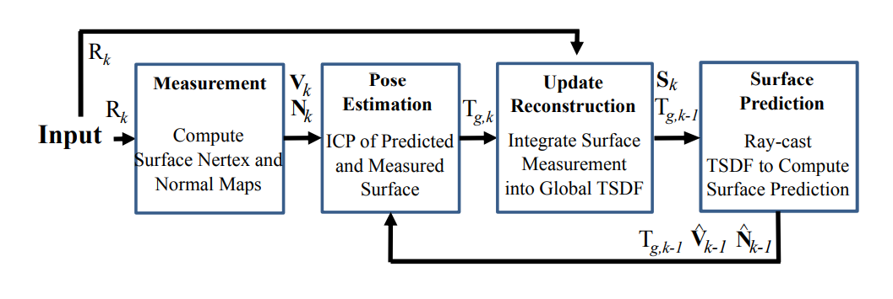
\includegraphics[scale=0.5]{figure1.png} %中括号中的参数是设置图片充满文档的大小,你也可以使用小数来缩小图片的尺寸。
    \caption{Overall system workflow\cite{6162880}.} %caption是用来给图片加上图题的
    \label{figure1} %这是添加标签,方便在文章中引用图片。
\end{figure}%figure环境

\subsection{Preliminaries}
The pose of the real-time camera from the current frame \textit{k} to the global frame \textit{g} can be represented by a rigid body transformation matrix:
\begin{equation}
	T_{g,k} = \left\{
	\begin{pmatrix}
	R_{g,k} & \mathbf{t_{g,k}} \\ \mathbf{0} & 1
	\end{pmatrix}
	:
	R_{g,k}^\top R_{g,k} = R_{g,k} R_{g,k}^\top = I_3, \mathbf{t_{g,k}}\in\mathbb{R}^3
	\right\},
	\label{equ1}
	\end{equation}
A point $ \mathbf{p_k}\in\mathbb{R}^3 $ in the camera frame is transferred into the global co-ordinate frame via $ \mathbf{p_g}=T_{g,k}\mathbf{p_k}$.
And the constant camera calibration matrix K converts the points of the camera coordinate system into the points of the pixel coordinate system.
The function $\mathbf{q}=\pi(\mathbf{p})$ performs the perspective projection of $\mathbf{p}\in\mathbb{R}^3=(x,y,z)^\top$, including de-homogenization to obtain $\mathbf{q}\in\mathbb{R}^2=(x/z,y/z)^\top$. 
This paper also uses dot notation to represent the homogeneous vector $\dot{\mathbf{u}}: =(\mathbf{u}^\top | 1)^\top$\cite{6162880}.

\subsection{Surface measurement}
In the $k$ frame, the measurement includes the original depth map $R_k$, and the calibrated depth measurement value $R_k(\mathbf{u})\in\mathbb{R}$ is provided on each image. 
The pixel is in the image domain $\mathbf{u}\in\mathbb{R}^2$, such that $\mathbf{p_k} = R_k(\mathbf{u})K^{-1}\dot{\mathbf{u}}$ is the measurement point in the reference $k$ frame.
The bilateral filter can be applied to the original depth map to obtain a discontinuity preserved depth map with reduced noise $D_k$,
\begin{equation}
	D_{k}(\mathbf{u}) = \frac{1}{W_\mathbf{p}}\sum_{\mathbf{q}}\mathcal{N}_{\sigma_{s}}(||\mathbf{u}-\mathbf{q}||_2)\mathcal{N}_{\sigma_{r}}(||R_k(\mathbf{u})-R_k(\mathbf{q})||_2)R_k(\mathbf{q}),
	\label{equ2}
\end{equation}
where $\mathcal{N}_{\sigma}(t) = \exp(-t^{2}\sigma^{-2})$ and $W_{\mathbf{p}}$ is a normalizing constant.
\begin{figure}[h] %figure环境,h默认参数是可以浮动,不是固定在当前位置。如果要不浮动,你就可以使用大写float宏包的H参数,固定图片在当前位置,禁止浮动。
    \centering %使图片居中显示
    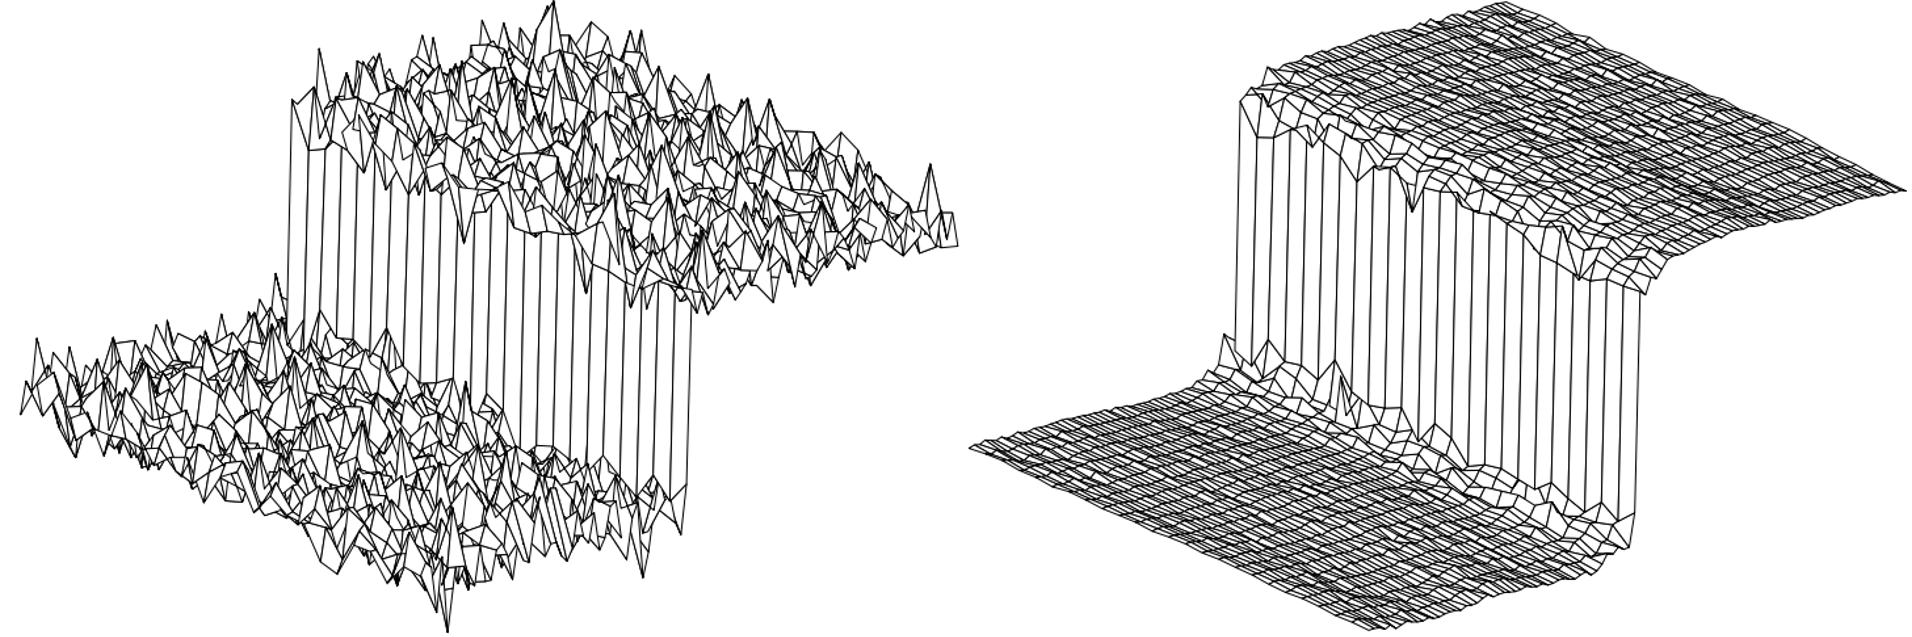
\includegraphics[scale=0.4]{figure2.png} %中括号中的参数是设置图片充满文档的大小,你也可以使用小数来缩小图片的尺寸。
    \caption{Result of denoising by bilateral filter\cite{710815}.} %caption是用来给图片加上图题的
    \label{figure2} %这是添加标签,方便在文章中引用图片。
\end{figure}%figure环境
\\The result of denoising is shown in the Figure \ref{figure2}. The bilateral filter can denoise the depth map while preserving the depth of the depth map.
\\The filtered depth values are back-projected to the frame of the reference to obtain the vertex map $\mathbf{V}_k$,
\begin{equation}
	\mathbf{V}_k(\mathbf{u}) = D_k(\mathbf{u})K^{-1}\dot{\mathbf{u}}
	\label{equ3}
\end{equation}
\\The cross product between adjacent map vertices can be used to calculate the corresponding normal vector,
\begin{equation}
	\mathbf{N}_k(\mathbf{u}) = {\rm v}[(\mathbf{V}_k(u+1,v)-\mathbf{V}_k(u,v))\times(\mathbf{V}_k(u,v+1)-\mathbf{V}_k(u,v))],
	\label{equ4}
\end{equation}
where ${\rm v}[\mathbf{x}] = \mathbf{x}/||\mathbf{x}||_2$.
\\The vertex and normal map pyramid need to be built as a multi-scale representation of the surface measurement. 
Setting the bottom depth map pyramid level equal to the original bilateral filtered depth map, the sub-sampled version $D^{l+1}$ is computed from $D^l$ by block averaging followed by sub-sampling to half the resolution. 
Then each level in a vertex and normal map pyramid $\mathbf{V}^{l\in[1...L]}$, $\mathbf{N}^{l\in[1...L]}$ is computed with Equations \ref{equ3} and \ref{equ4} using the corresponding depth map level.
\subsection{Pose estimation}
The key concepts of the standard ICP algorithm can be summarized in two steps\cite{inproceedings}:
\begin{itemize}
	\item[1.] Calculate the correspondence between two point sets.
	\item[2.] Calculate the transformation between corresponding points to minimize the distance.
\end{itemize}
Because the corresponding relationship of the point sets may not be completely correct, we need to iteratively obtain the new corresponding relationship to calculate the desired transformation. 
\\There are many ways to calculate the distance of the ICP algorithm. In KinectFusion, we use the global point-to-plane distance. 
Point-to-plane distance considers sum of the squared distance between each source point and the tangent plane at its corresponding destination point (see Figure \ref{figure4}).
Compared with the point-to-point distance, point-to-plane distance considers the local structure of the point cloud, which has higher accuracy and is not easy to fall into the local optimum. 
if $\mathbf{s_i}$ is a source point, $\mathbf{d_i} $ is the corresponding destination point, and $\mathbf{n_i}$ is the unit normal vector at $\mathbf{d_i}$.
The global point-plane ICP formula is as follows\cite{article},
\begin{equation}
	\mathbf{M}_{opt} = \arg\min_{\mathbf{M}}\sum_i(\mathbf{(M\cdot s_i-d_i)\cdot n_i})^2,
	\label{equ5}
\end{equation}
where $\mathbf{M}$ and $\mathbf{M}_{opt}$ are 4×4 3D rigid-body transformation matrices.
\begin{figure}[h] %figure环境,h默认参数是可以浮动,不是固定在当前位置。如果要不浮动,你就可以使用大写float宏包的H参数,固定图片在当前位置,禁止浮动。
    \centering %使图片居中显示
    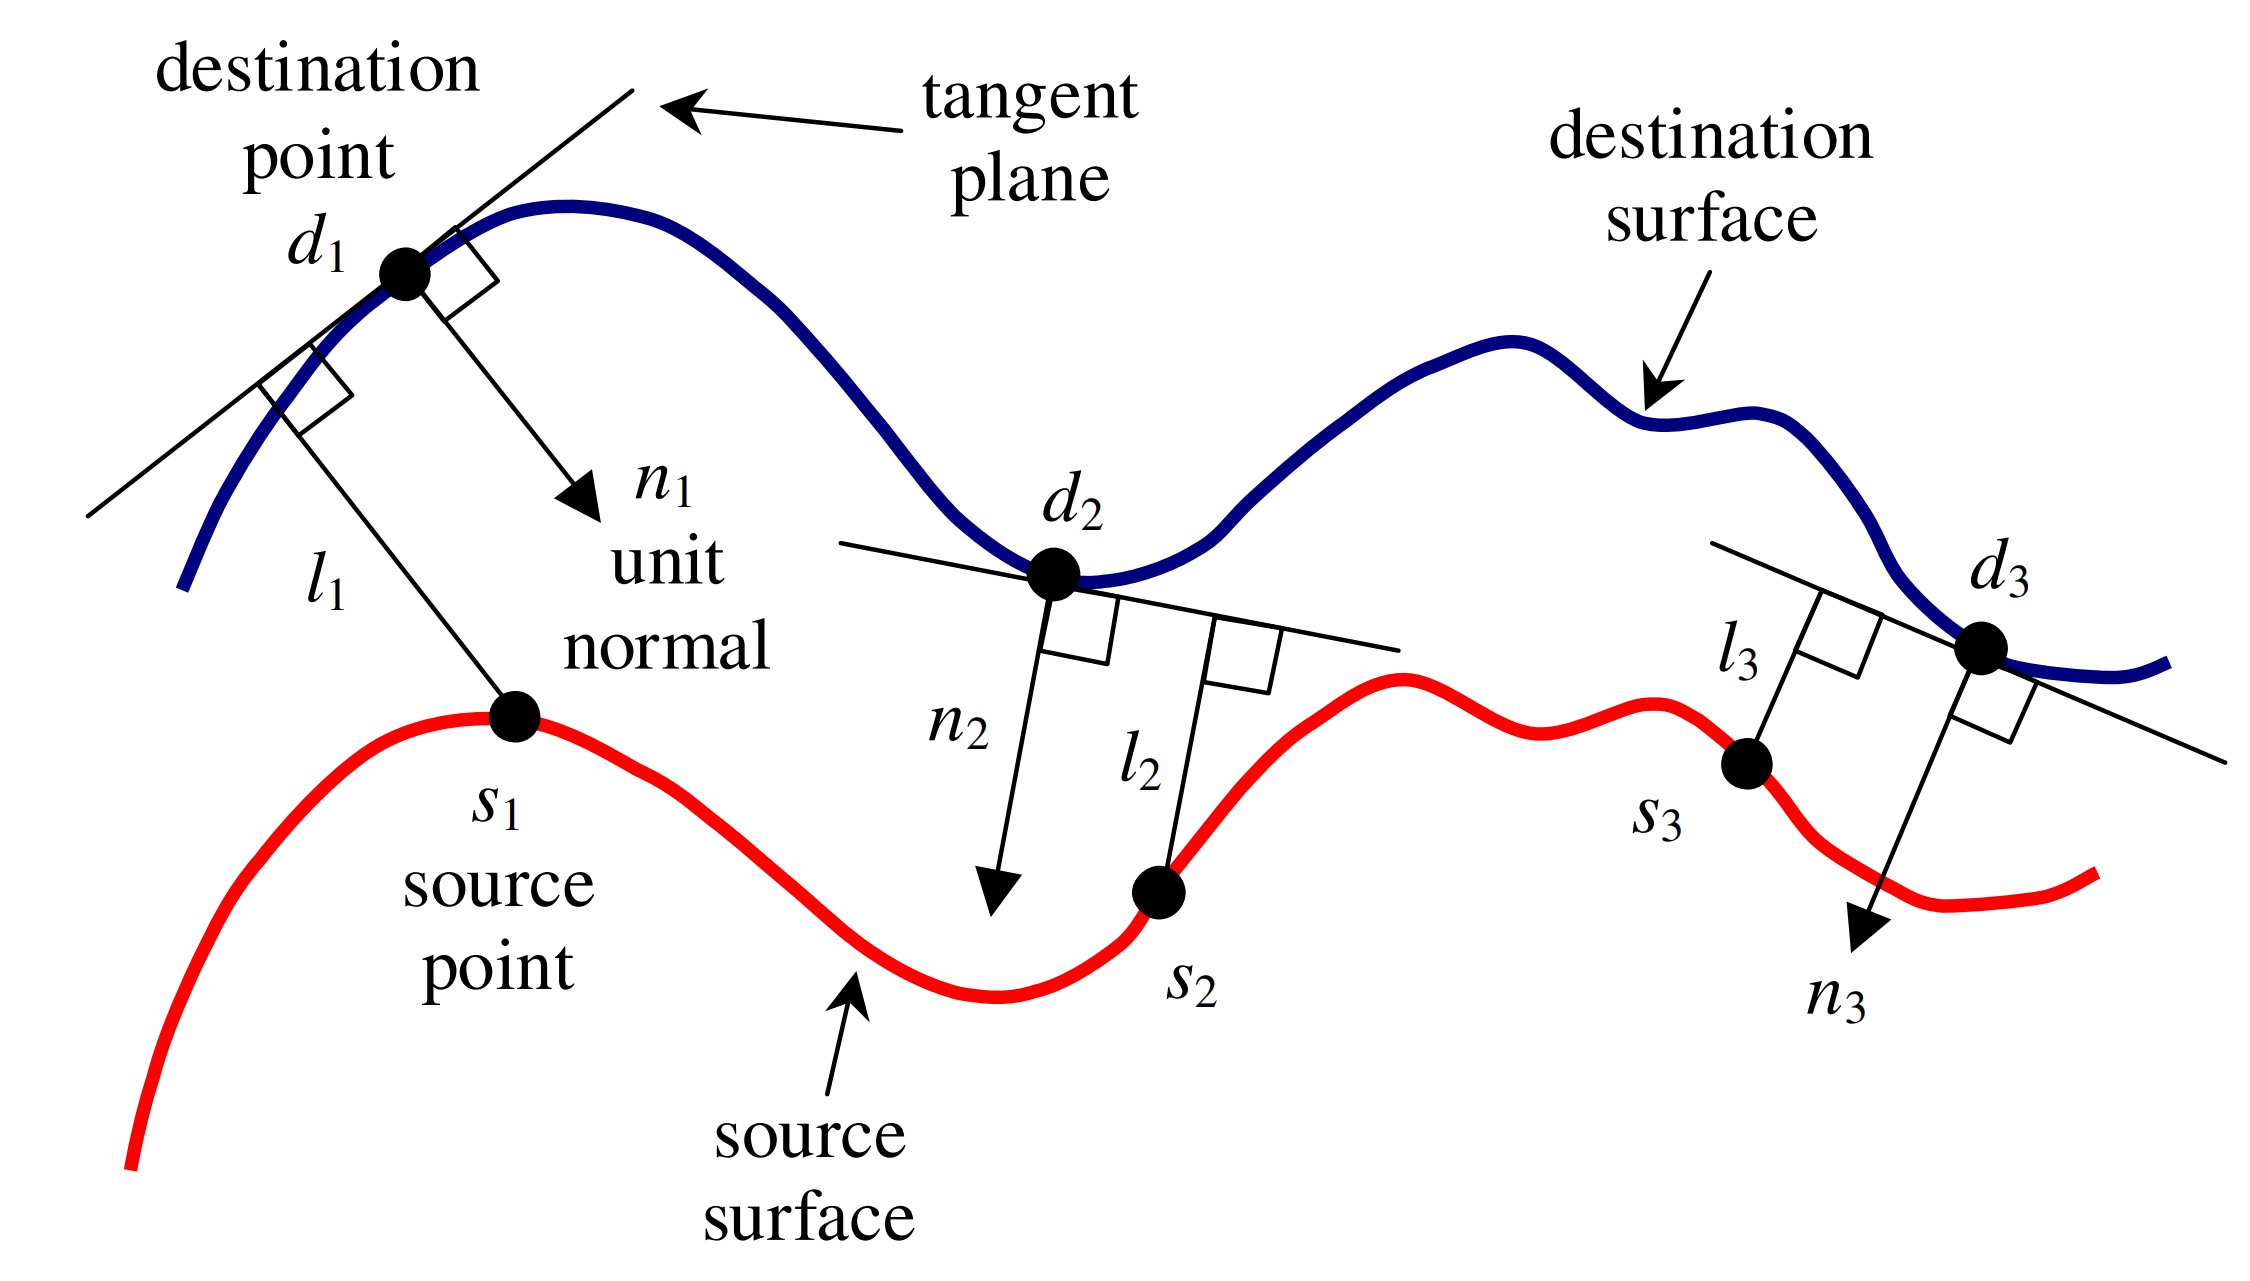
\includegraphics[scale=0.3]{figure4.png} %中括号中的参数是设置图片充满文档的大小,你也可以使用小数来缩小图片的尺寸。
    \caption{Point-to-plane error between two surfaces\cite{article}.} %caption是用来给图片加上图题的
    \label{figure4} %这是添加标签,方便在文章中引用图片。
\end{figure}%figure环境
\\Using the ICP algorithm, we can estimate the rotation and translation of the current frame. 
Applying the Equation \ref{equ5} of global point-plane ICP, we can obtain the following expression,
\begin{equation}
	\mathbf{E}(T_{g,k}) = \sum||(T_{g,k}\mathbf{\dot{V}}_k(u)-\mathbf{\hat{V}}_{k-1}^g(\mathbf{\hat{u}}))^\top\mathbf{\hat{N}}_{k-1}^g(\hat{\mathbf{u}})||_2,
	\label{equ6}
\end{equation} 
where $\mathbf{u}$ is the pixel of the current frame, $\mathbf{\hat{V}}_{k-1}^g$, and $\mathbf{\hat{N}}_{k-1}^g$ are the vertex map and normal map of the surface prediction in the global model built from all $k-1$ frames.
$\mathbf{\hat{u}}=\pi(K\tilde{T}_{k-1,k}\mathbf{\dot{V}}_k(\mathbf{u}))$ is the result of projecting the pixel of the current frame to the $k-1$ frame through rotation and translation using an estimate for the frame-frame transformation $\tilde{T}_{k-1,k}^z=\tilde{T}_{g,k-1}^{-1}\tilde{T}_{g,k}^z$. 
The frame-frame transformation matrix $\tilde{T}_{k-1,k}^z$ here contains the current transformation matrix $\tilde{T}_{g,k}^z$ that we need to solve, so the correspondence between pixels $\mathbf{u}$ and $\mathbf{\hat{u}}$ may not be correct. 
We need to iteratively solve the transformation matrix, and $z$ means the number of iterations.
\\Although we have expressed the function to be optimized, this function is not in the form of linear least squares and it is difficult to optimize. Now, the objective function of ICP needs to be transformed into the form of linear least squares.
The camera pose is obtained continuously through incremental matrix $\tilde{T}_{inc}^z$ by iteration. In each iteration, the pose matrix is continuously multiplied by the incremental matrix($\tilde{T}_{g,k}^z=\tilde{T}_{inc}^z\tilde{T}_{g,k}^{z-1}$), and the new matrix continuously approaches the real camera pose.
The increment matrix can be written in the following form with the small-angle assumption,
\begin{equation}
	\tilde{T}_{inc}^z = 
	\begin{bmatrix}
		\tilde{R}^z | \tilde{\mathbf{t}}^z 
	\end{bmatrix}
	=
	\begin{bmatrix}
		1&\alpha&-\gamma&t_x\\-\alpha&1&\beta&t_y\\\gamma&-\beta&1&t_z
	\end{bmatrix}.
	\label{equ7}
\end{equation}
\\If the rigid body transformation matrix is written in the form of twist coordinate, the first term($T_{g,k}\mathbf{\dot{V}}_k(u)$) with respect to the iteration $z$ of the Equation \ref{equ6} can be written as a linear relationship to $\mathbf{x}=(\beta,\gamma,\alpha,t_x,t_y,t_z)^\top$,
\begin{equation}
	\tilde{T}_{g,k}^z\mathbf{\dot{V}}_k(\mathbf{u}) =\tilde{R}^z\mathbf{\tilde{V}}_k^g(\mathbf{u})+\tilde{\mathbf{t}}^z=\mathbf{G(u)x}+\mathbf{\tilde{V}}_k^g(\mathbf{u}),
	\label{equ8}
\end{equation} 
where the 3×6 matrix $\mathbf{G}$ is formed with the skew-symmetric matrix form of $\tilde{V}_{k}^{g}(\mathbf{u})$:
\begin{equation}
	\mathbf{G(u)} =
	\begin{bmatrix}
		\tilde{V}_{k}^{g}(\mathbf{u})_\times | \mathbf{t}_{3\times3}.
	\end{bmatrix}
	\label{equ9}
\end{equation}
and $\tilde{V}_{k}^{g}(\mathbf{u})=\tilde{T}_{g,k}^{z-1}\mathbf{\dot{V}}_k(\mathbf{u})$.
\\An iteration is obtained by solving:
\begin{equation}
	\min_{\mathbf{x}}\sum||E||_2^2
	\label{equ10}
\end{equation} 
\begin{equation}
	E=\mathbf{\hat{N}}_{k-1}^g(\hat{\mathbf{u}})^\top(\mathbf{G(u)x}+\mathbf{\tilde{V}}_k^g(\mathbf{u})-\mathbf{\tilde{V}}_{k-1}^g(\mathbf{\hat{u}}))
	\label{equ11}
\end{equation}
\\Finally, the objective function $E$ is expressed in a linear form, and it satisfies the First-order optimality condition, $\mathbf{x}$ can be obtained as follows:
\begin{align}
	\sum\mathbf{(A^\top A)x}&=\sum\mathbf{A^\top b},\\
	\mathbf{A^\top}&=\mathbf{G^\top(u)}\mathbf{\hat{N}}_{k-1}^g(\mathbf{\hat{u}}),\\
	\mathbf{b}&=\mathbf{\hat{N}}_{k-1}^g(\mathbf{\hat{u}})^\top(\mathbf{\tilde{V}}_k^g(\mathbf{\hat{u}})-\mathbf{\tilde{V}}_{k-1}^g(\mathbf{u})).
\end{align}

The data association and pose minimisation is embedded into a coarse to fine framework using the bottom 3 levels of a vertex and normal map pyramid. 
We iterate for a maximum of $z_{max}$ = [4,5,10] iterations in levels [3,2,1] respectively, starting with the coarsest level 3.
In this paper, the problem is highly non-convex. Our algorithm for pose estimation can easily fall into a local optimum. 
Therefore, a good initialization is very useful to obtain the global optimum.
The image pyramid is a scheme from coarse to fine, which can provide good initialization for optimization from coarse level to fine level, which can help us solve the initialization problem.

\subsection{Surface reconstruction update}
In the third part we need to update the reconstruction with the pose, here we use TSDF(truncated signed distance function).
It is a representation method of the 3D map. It uses a large volume. The volume is composed of many small voxels. Each voxel corresponds to a point in space. 
Two components are stored at each location of the TSDF: the current truncated signed distance value $F_k(\mathbf{p})$ and a weight $W_k(\mathbf{p})$,
\begin{equation}
	\mathbf{S}_k(\mathbf{p}) \mapsto[F_k(\mathbf{p}),W_k(\mathbf{p})].
	\label{equ15}
\end{equation}
Through the following formula,
\begin{align}
	F_k(\mathbf{p})&=\Psi(\lambda^{-1}||\mathbf{t}_{g,k}-\mathbf{p}||_2-R_k(\mathbf{x})),\\
	\lambda&=||K^{-1}\dot{\mathbf{x}}||_2,\\
	\mathbf{x}&=\lfloor\pi(KT_{g,k}^{-1}\mathbf{p})\rfloor,\\
	\Psi(\eta)&=
	\left\{
		\begin{array}{lr}
		\min(1,\dfrac{\eta}{\mu})\text{sgn}(\eta) & \text{iff } \eta\geq-\mu \\
		null & otherwise
	\end{array}
	\right.
\end{align}
where $\lfloor\cdot\rfloor$ is a nearest neighbour lookup, instead of interpolating the depth value,
1/$\lambda$ converts the ray distance to $\mathbf{p}$ to a depth, $\Psi$ performs the SDF
truncation, the weight $W_k(\mathbf{p})$ is related to the uncertainty of surface measurement,
we can calculate the TSDF value of each voxel.
If the value is greater than or less than the threshold, it will be truncated to 1 or -1. Only the TSDF value near the surface will be accurately represented as shown in Figure \ref{figure5} .
\begin{figure}[h] %figure环境,h默认参数是可以浮动,不是固定在当前位置。如果要不浮动,你就可以使用大写float宏包的H参数,固定图片在当前位置,禁止浮动。
    \centering %使图片居中显示
    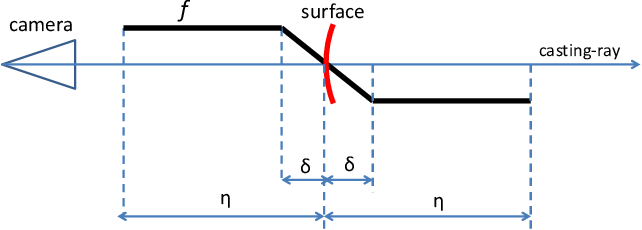
\includegraphics[scale=0.4]{figure5.png} %中括号中的参数是设置图片充满文档的大小,你也可以使用小数来缩小图片的尺寸。
    \caption{Illustration of the truncated signed distance function\cite{Kang2014FastD3}.} %caption是用来给图片加上图题的
    \label{figure5} %这是添加标签,方便在文章中引用图片。
\end{figure}%figure环
\\The global fusion of all depth maps in the volume is formed by the weighted average of all individual TSDF, which can be seen as de-noising the global TSDF from multiple noisy TSDF measurements:
\begin{equation}
	\min\sum||W_{R_k}F_{R_k}-F||_2.
	\label{equ16}
\end{equation}
Since our focus is on real-time sensor tracking and surface reconstruction, we continue to integrate the new TSDF measurement into the global TSDF measurement:
\begin{align}
	F_k(\mathbf{p})&=\frac{W_{k-1}(\mathbf{P})F_{k-1}(\mathbf{P})+W_{R_k}(\mathbf{P})F_{R_k}(\mathbf{P})}{W_{k-1}(\mathbf{P})+W_{R_k}(\mathbf{P})},\\
	W_k(\mathbf{p})&=W_{k-1}(\mathbf{P})+W_{R_k}(\mathbf{P}).
\end{align}
\subsection{Surface prediction}
In the last step, we can construct a new global vertex map $\hat{\mathbf{V}}_k^g(\mathbf{u})$ and normal map $\hat{\mathbf{N}}_k^g(\mathbf{u})$ for the second step based on the current global TSDF reconstruction.
This paper uses the ray casting method. 
The ray, $T_{g,k}K^{-1}\dot{\mathbf{u}}$, starts from the minimum depth of each pixel $\mathbf{u}$ and follows direction until it encounters the zero-crossing($F_k(\mathbf{p})=0$), and the value of TSDF changes from positive to negative. 
We find the points of the surface based on the zero-crossing position and added them to the global vertex map $\mathbf{\hat{V}}_k$.
\\and the surface normal for the associated pixel $\mathbf{u}$ along which $\mathbf{p}$ was found can be computed directly from $F_k$ using a numerical derivative of the SDF:
\begin{equation}
	R_{g,k}\hat{\mathbf{N}}_k=\hat{\mathbf{N}}_k^g(\mathbf{u})=\text{v}[\nabla F(\mathbf{p})],\nabla F=\left[ \frac{\partial F}{\partial x},\frac{\partial F}{\partial y},\frac{\partial F}{\partial z} \right]^\top
	\label{equ17}
\end{equation}
\section{Experiments and results}

In our experiments, the Kinect sensor is placed in a fixed position to observe the desktop scene installed on the turntable. 
Then the depth data is captured in approximately 19 seconds, so that the turntable rotates a full circle, resulting in $N = 560$ frames. 
All parameters of the system are kept constant using a reconstruction resolution of $256^3$ voxels unless stated otherwise.
\\The N frames of depth data captured were then processed in each of the following ways:
\begin{itemize}
	\item[1.] Frames $1...N$ were fused together within the TSDF using sensor pose estimates obtained with frame-to-frame ICP implementation.
	\item[2.] Frames $1...L, L < N$ were fed through our standard tracking and mapping pipeline. Here, sensor pose estimates are obtained by the full frame-model ICP method.
	\item[3.] Frames $1...N$ were fed through our standard tracking and mapping pipeline. Sensor pose estimates are obtained by frame-model ICP.
	\item[4.] Frames $1...N$ were fed repeatedly for $M = 4$ loops to the standard tracking and mapping pipeline. Sensor pose estimates are obtained by frame-model ICP.
\end{itemize}
\begin{figure}[h] %figure环境,h默认参数是可以浮动,不是固定在当前位置。如果要不浮动,你就可以使用大写float宏包的H参数,固定图片在当前位置,禁止浮动。
    \centering %使图片居中显示
    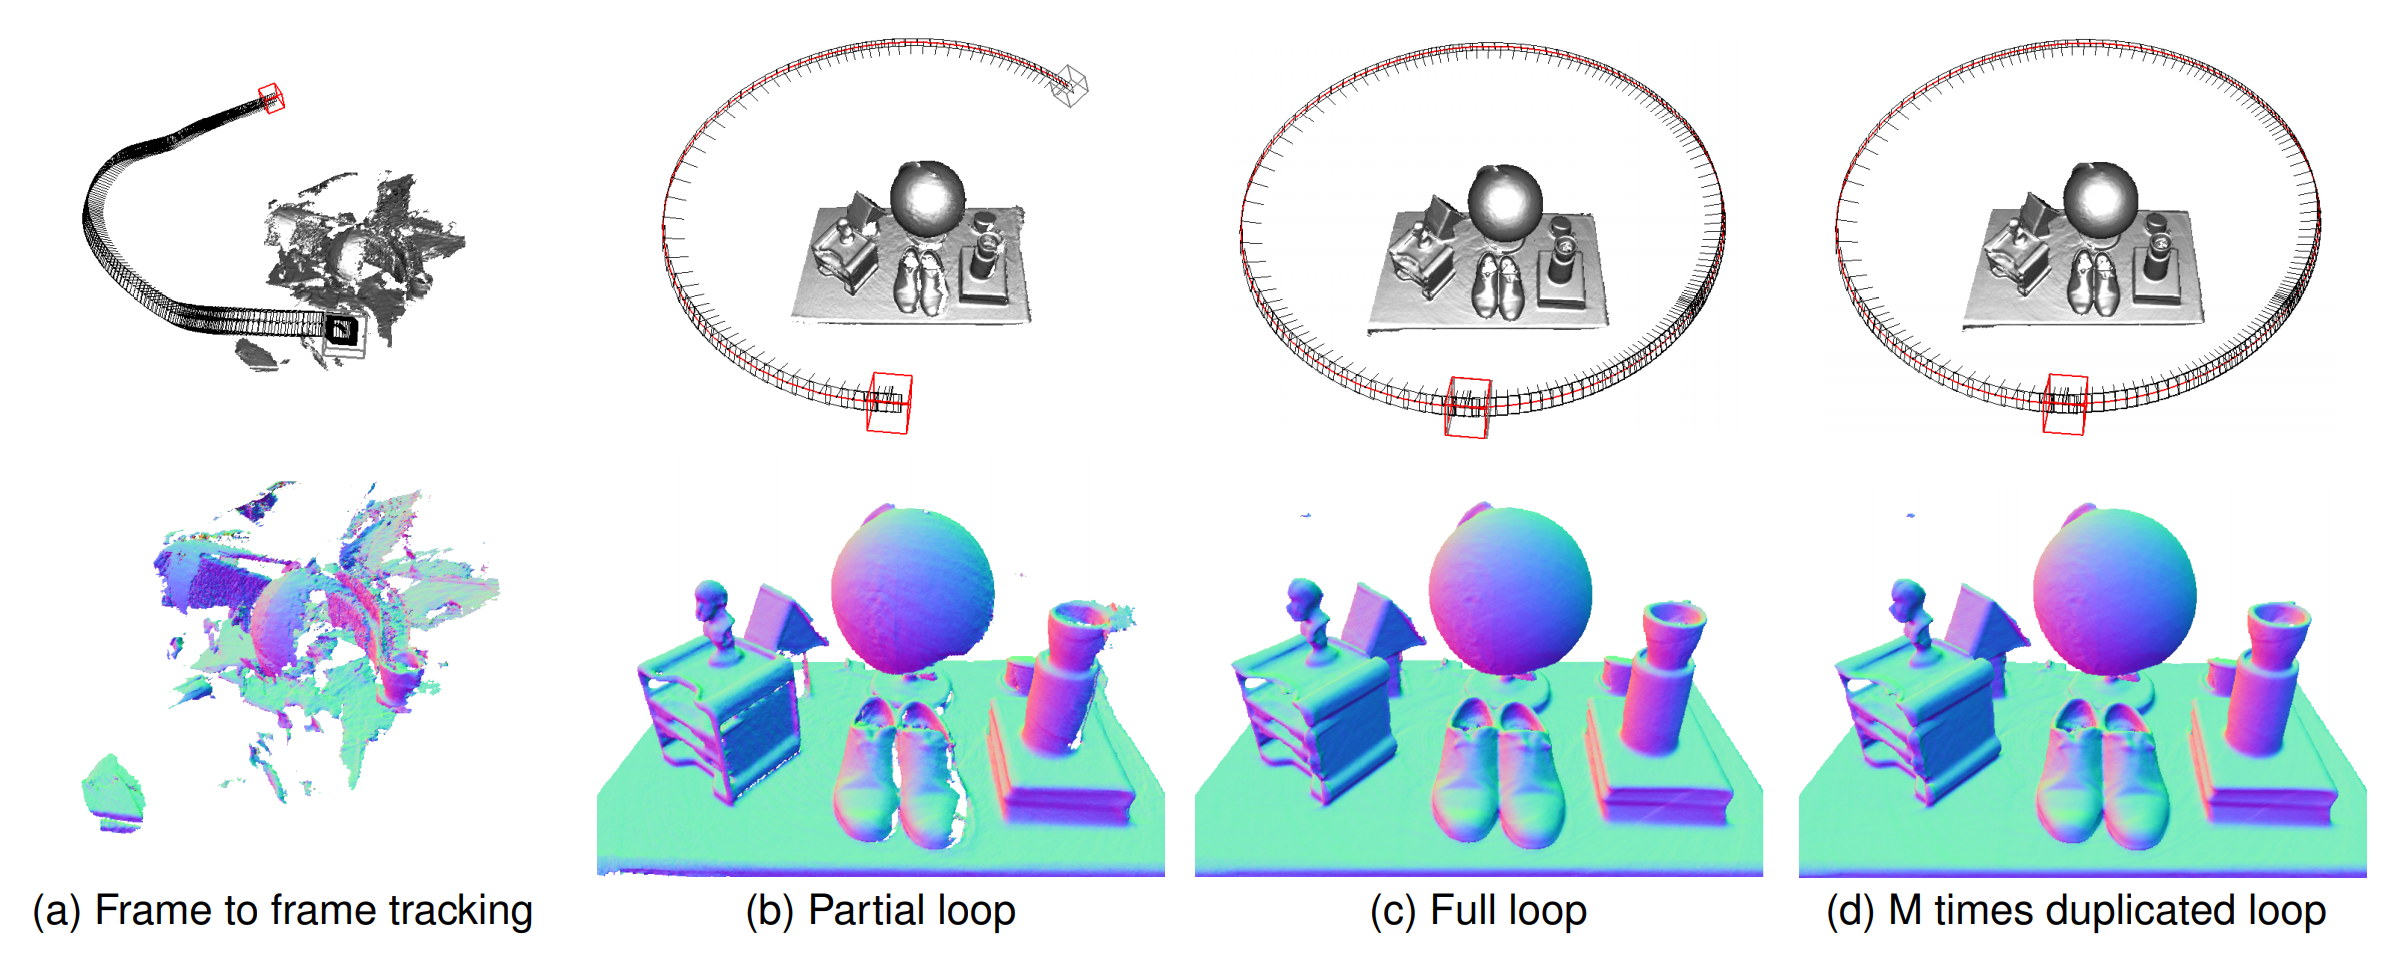
\includegraphics[scale=0.45]{figure6.png} %中括号中的参数是设置图片充满文档的大小,你也可以使用小数来缩小图片的尺寸。
    \caption{Circular motion experiment of our system as the sensor orbits a table\cite{6162880}.} %caption是用来给图片加上图题的
    \label{figure6} %这是添加标签,方便在文章中引用图片。
\end{figure}%figure环
(a), frame-to-frame tracking, the pose of each new frame is estimated by just the last frame. Rapid accumulation of errors results in the non-circular trajectory and poor reconstruction is apparent.
(b)(c)(d) show our full frame-to-model tracking approach. 
From (b)(c)(d), we can obtain better 3D reconstruction results using our frame-to-model tracking approach.
\begin{figure}[h] %figure环境,h默认参数是可以浮动,不是固定在当前位置。如果要不浮动,你就可以使用大写float宏包的H参数,固定图片在当前位置,禁止浮动。
    \centering %使图片居中显示
    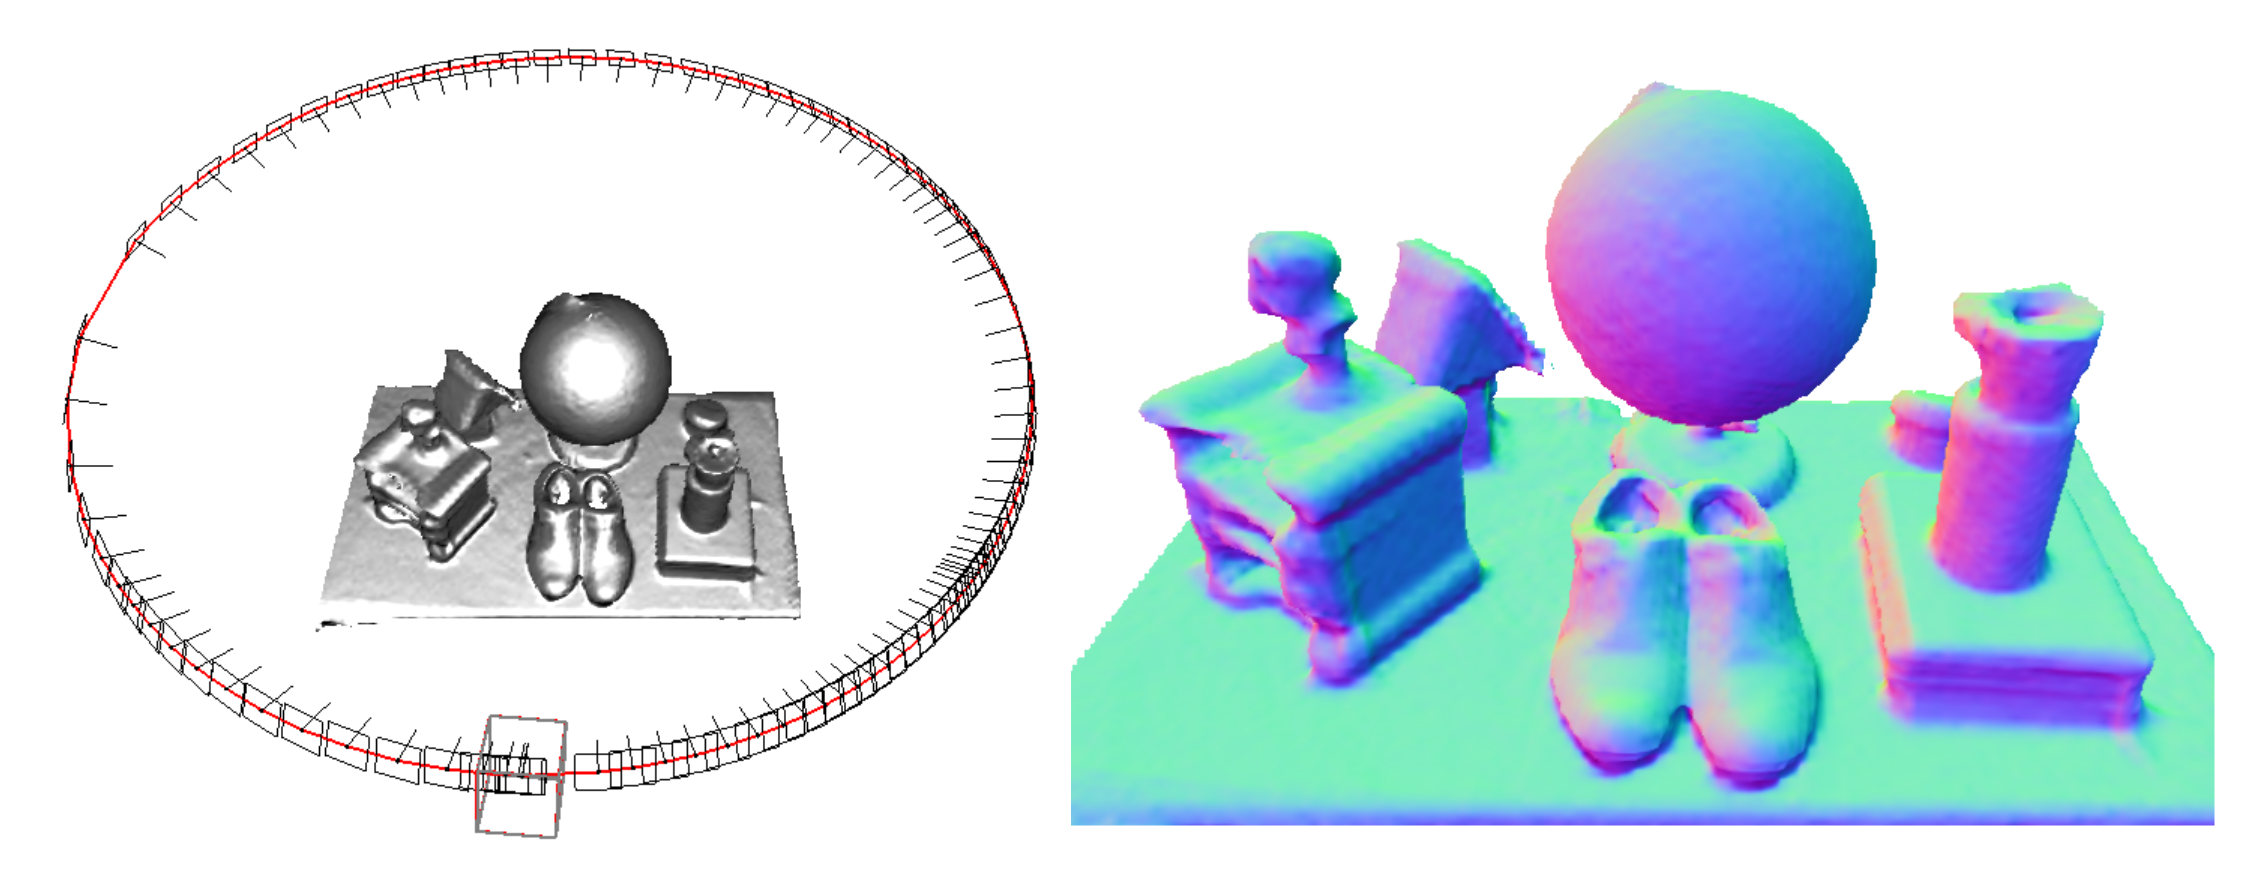
\includegraphics[scale=0.35]{figure7.png} %中括号中的参数是设置图片充满文档的大小,你也可以使用小数来缩小图片的尺寸。
    \caption{A reconstruction result using $\frac{1}{64}$ the memory of the Figure \ref{figure6}, and using only every $6_{th}$ sensor frame\cite{6162880}.} %caption是用来给图片加上图题的
    \label{figure7} %这是添加标签,方便在文章中引用图片。
\end{figure}%figure环
\\Figure \ref{figure7} shows the reconstruction result where the the $N$ frames are sub-sampled in time to use every $6_{th}$ frame, and 64 times less GPU memory is used by reducing the reconstruction resolution to $64^3$.
The computing and storage resources required to build the model have been greatly reduced, but the reconstruction quality has not dropped significantly.

\section{Discussion / Conclusion}
Compared with the frame-to-frame model, our frame-to-model system can obtain high-quality reconstruction results through the above experiment, even in the case of low resolution. 
But our model page has a main failure, our model is difficult to reconstruct a very large plane. The reason is that we use the global point-plane ICP algorithm to estimate the pose of the camera.
one possible solution is to add photometric cost.
\\In this work, we implemented a real-time tracking and mapping method from frame to model. The key concepts in our real-time tracking and mapping system are:
\begin{itemize}
	\item Up-to-date surface representation fusing all registered data from previous scans.
	\item Accurate and robust tracking of the camera pose by aligning all depth points with the complete scene model.
	\item Parallel algorithms for both tracking and mapping, taking full advantage of commodity GPU processing hardware.
\end{itemize}
A interesting direction is to reconstruct a large model.
The current method is only suitable for drawing small rooms. However, rebuilding large models (such as entire buildings) adds many other challenges. 
The current dense volume representation will require too much memory and more space, and will cause inevitable drift.


\bibliographystyle{plain}
\bibliography{report}

\end{document}